\documentclass[11pt,a4paper]{article}

\usepackage[T1]{fontenc}
\usepackage[utf8]{inputenc}
\usepackage{lmodern}
\usepackage[margin=2.5cm]{geometry}
\usepackage{amsmath,amssymb}
\usepackage{booktabs}
\usepackage{tabularx}
\usepackage{graphicx}
\usepackage{xcolor}
\usepackage{algorithm}
\usepackage{algpseudocode}
\usepackage{enumitem}
\usepackage[hidelinks]{hyperref}
\usepackage{cleveref}
\usepackage{caption}
\usepackage{makecell}

\newcommand{\code}[1]{\texttt{#1}}
\newcommand{\pending}{\textit{pending}}
\setlist{itemsep=2pt,topsep=4pt}
\emergencystretch=3em

\title{\textbf{scx\_hush: Unfair-by-Design CPU Scheduling\\for Mixed Latency-Critical and Background Workloads\\with \code{sched\_ext}}}
\author{Mohak\\[2pt]\small Technical report, \today}
\date{}

\begin{document}
\maketitle

\begin{abstract}
General-purpose operating systems schedule CPU time by proportional share.
Lowering the priority of background work (nice values, \code{SCHED\_IDLE},
cgroup \code{cpu.idle}) shrinks its share but never removes it, so
deferrable jobs such as compilation, compression or database maintenance
still delay latency-critical foreground work. Strict prioritisation removes
that interference but brings two new failure modes: unbounded starvation and
priority inversion through shared locks. We present \emph{scx\_hush}, a CPU
scheduler for Linux, loaded at runtime through the extensible scheduler class
\code{sched\_ext}. It gives foreground work strict precedence and preempts
background work as soon as foreground work wakes. A rate-limited starvation
guard bounds how long background work waits. Priority inversion is resolved
with four detection tiers (application hints, PI futexes, glibc mutexes and
uninterruptible-sleep escape) plus a same-process fallback. Classification
comes from cgroups, process names and user IDs in a policy file, so
unmodified applications benefit. scx\_hush generalises the database-specific
UFS design~\cite{ufs2026} to any machine that mixes the two kinds of work.
This report describes the design, a complete implementation (about 6{,}100
lines of BPF, C and Python, excluding tests), its verification, and an evaluation methodology
with nine experiments. Baseline measurements on a 4-vCPU machine confirm the interference
the design targets: under CPU-bound background load, the p99 wakeup latency
of a foreground benchmark rose about $49\times$ with the default scheduler,
and neither nice~19 nor \code{SCHED\_IDLE} reduced it. The in-kernel evaluation of scx\_hush itself
requires a \code{sched\_ext}-enabled kernel and is left as the immediate next
step; no scx\_hush performance figures are claimed here.
\end{abstract}

\section{Introduction}
\label{sec:intro}

Many machines run two kinds of work at once. One kind is something a person
or a control loop is waiting on: a video call, an editor, a robot's 100\,Hz
control loop, the query threads of a database. The other kind is deferrable
bulk work: a parallel compiler build, log compression, a backup,
\code{VACUUM}. \Cref{tab:usecases} lists representative settings.

\begin{table}[h]
\centering\small
\caption{The two-class pattern on different machines.}
\label{tab:usecases}
\begin{tabularx}{\linewidth}{@{}lXXX@{}}
\toprule
Setting & Foreground (latency-critical) & Background (deferrable) & Symptom today \\
\midrule
Developer laptop & compositor, editor, video call & compiler builds, indexing, backups & UI stutter, dropped frames \\
Robot / drone computer & perception, planning, control loop & log compression, map building, upload & control-loop jitter \\
Database server & query and request threads & vacuum, compaction, analytics & tail latency doubles in maintenance windows \\
Shared lab / CI machine & interactive SSH, notebooks & long training or test jobs & interactive sessions unusable \\
\bottomrule
\end{tabularx}
\end{table}

\paragraph{Problem statement.}
Linux offers several priority mechanisms: nice values, the \code{SCHED\_IDLE}
policy and cgroup CPU weights including \code{cpu.idle}. All of them are
proportional-share mechanisms. A background task at the lowest weight still
receives slices. It still occupies a CPU when a foreground task wakes, so the
foreground task waits for the next scheduling decision. And it can still hold
a lock that a foreground task needs. The UFS authors show that OS schedulers,
despite supporting priorities, do not reliably isolate high-priority tasks,
and remain vulnerable to priority inversion~\cite{ufs2026}.
The problem this work addresses is:

\begin{quote}
\emph{How can a general-purpose machine run deferrable background work only
on CPU time that latency-critical foreground work does not want, without
modifying applications, while bounding background starvation and resolving
priority inversion, and with no risk to system stability?}
\end{quote}

\paragraph{Contributions.}
\begin{enumerate}
\item A survey of proportional-share, colocation, user-space and pluggable
  scheduling approaches, and five research gaps that they leave
  (\cref{sec:related}).
\item The design of scx\_hush: strict class ordering with immediate
  preemption, a watchdog-safe starvation guard, and a four-tier
  priority-inversion mechanism with bounded, capped boosts
  (\cref{sec:design}).
\item A complete implementation on \code{sched\_ext}: the BPF scheduler, a
  C daemon and loader, a CLI, a hint library and an evaluation harness
  (\cref{sec:impl}).
\item A reproducible evaluation methodology of nine experiments against six
  baselines and one ablation. We report verification results and baseline
  measurements, and state clearly which results are still outstanding
  (\cref{sec:eval,sec:results}).
\end{enumerate}

\section{Background}
\label{sec:background}

\paragraph{Proportional-share scheduling in Linux.}
Linux's fair class orders runnable tasks by weighted virtual runtime. The
Completely Fair Scheduler did this from 2.6.23, and EEVDF~\cite{stoica1995eevdf}
has done so since 6.6. Nice values change a task's weight: nice~19 weighs
15, against 1024 at nice~0. \code{SCHED\_IDLE} gives a task the minimum
weight, and cgroup v2 \code{cpu.idle}~\cite{cgroupv2-docs} gives a whole group
idle-class treatment. In all three cases, low priority means a small share,
not ``none while foreground is runnable''.

\paragraph{sched\_ext.}
The extensible scheduler class~\cite{schedext-docs}, merged in Linux 6.12,
lets a BPF program implement \code{struct sched\_ext\_ops}. Tasks flow through
\emph{dispatch queues} (DSQs): one global FIFO, one local DSQ per CPU, and
any number of custom DSQs, which can be FIFOs or virtual-time priority queues.
A CPU runs the head of its local DSQ. When that is empty, the CPU calls
\code{ops.dispatch()}. Safety is built in: a BPF error, a runnable task left
unscheduled past a watchdog timeout (at most 30\,s), or SysRq-S aborts the
BPF scheduler and returns every task to the fair class. The kernel
documentation warns that \code{sched\_ext} kfuncs carry no ABI stability
guarantee. For example, \code{scx\_bpf\_dispatch} has been renamed to
\code{scx\_bpf\_dsq\_insert}.

\paragraph{Priority inversion and futexes.}
Priority inversion occurs when a high-priority task waits for a resource held
by a lower-priority task. Priority inheritance~\cite{sha1990pip} temporarily
raises the holder's priority until it releases the resource. User-space locks
on Linux are built on futexes~\cite{franke2002futex}. PI futexes
(\code{FUTEX\_LOCK\_PI}) keep the owner's thread ID in the futex word as
kernel ABI. Default glibc mutexes use \code{FUTEX\_WAIT} and record the owner
in a separate \code{\_\_owner} field. Strict prioritisation makes inversion
worse, not better: a low-priority holder may never run at all.

\section{Literature Review}
\label{sec:related}

\paragraph{Proportional-share schedulers.}
Lottery~\cite{waldspurger1994lottery} and stride~\cite{waldspurger1995stride}
scheduling established proportional share as a flexible resource abstraction.
EEVDF~\cite{stoica1995eevdf} added deadlines for accuracy, and it is now
Linux's default. BVT~\cite{duda1999bvt} let latency-sensitive threads
\emph{borrow} virtual time to dispatch early, so it gives low latency inside a
fair-share framework. All of these schedulers, however, keep giving
low-weight work a share by design. Lozi et~al.~\cite{lozi2016wasted} showed
further that Linux's general-purpose balancing logic can leave cores idle
while work waits, and that scheduler correctness is hard to get right, which
motivates making new policies safe to deploy.

\paragraph{Real-time scheduling.}
\code{SCHED\_DEADLINE}~\cite{lelli2016deadline} and PREEMPT\_RT provide hard
guarantees. They require per-task timing parameters and careful admission
control, so they do not fit unmodified desktop or server applications.
scx\_hush targets soft real-time behaviour and leaves hard guarantees out of
scope.

\paragraph{Colocation of latency-critical and best-effort work.}
Datacenter systems colocate latency-critical (LC) services with best-effort
batch jobs to raise utilisation. Borg~\cite{verma2015borg} separates
production and batch priorities across a cluster. Heracles~\cite{lo2015heracles}
and PARTIES~\cite{chen2019parties} partition cores, cache, memory bandwidth and
power using feedback control on LC latency. These systems work at coarse
granularity: they adjust allocations over seconds, rather than deciding every
context switch.

\paragraph{Microsecond-scale and user-space scheduling.}
Shinjuku~\cite{kaffes2019shinjuku} uses preemption at microsecond intervals to
cut tail latency. Shenango~\cite{ousterhout2019shenango} and
Caladan~\cite{fried2020caladan} reallocate cores between LC and batch
applications at microsecond timescales. These systems deliver excellent tail
latency, but they need applications built on their runtimes or kernel-bypass
stacks.

\paragraph{Pluggable kernel scheduling.}
ghOSt~\cite{humphries2021ghost} delegates Linux scheduling decisions to a
user-space agent. Syrup~\cite{kaffes2021syrup} lets applications supply
scheduling policies, written in eBPF~\cite{mccanne1993bpf}, across the stack.
\code{sched\_ext}~\cite{schedext-docs,scx-project} is the upstream mechanism:
the policy runs as verified BPF inside the kernel and falls back to the
default scheduler on failure. Recent work applies \code{sched\_ext} to
resource control for AI agents~\cite{agentcgroup2026} and to LLM-generated
policies~\cite{agenticos2026}. Bechberger~\cite{bechberger2025} gives a
practical introduction.

\paragraph{Lock-holder preemption.}
Descheduling a lock holder is a known pathology in virtualised systems.
Uhlig et~al.~\cite{uhlig2004lhp} studied lock-holder preemption in
multiprocessor VMs and proposed making the hypervisor aware of locks held by
guests. Classic priority inheritance~\cite{sha1990pip} solves the problem for
kernel-visible locks with known priorities.

\paragraph{UFS: the direct basis.}
UFS~\cite{ufs2026} restricts background database tasks to idle CPU capacity
using an eBPF scheduler. It preempts them immediately when time-sensitive
tasks arrive, and handles priority inversion with application hints passed
through BPF maps. Integrated into PostgreSQL, UFS improved time-sensitive
throughput by up to $2\times$ and halved tail latency compared with existing
Linux options~\cite{ufs2026}. It is evaluated on a single application whose
code was modified to send hints.

\begin{table}[t]
\centering\small
\caption{Comparison of approaches. \checkmark\ = provided, $\circ$ = partial, --- = not provided.}
\label{tab:compare}
\begin{tabularx}{\linewidth}{@{}>{\raggedright\arraybackslash}p{4.2cm}>{\centering\arraybackslash}X>{\centering\arraybackslash}X>{\centering\arraybackslash}X>{\centering\arraybackslash}X>{\centering\arraybackslash}X@{}}
\toprule
Approach & \makecell{Strict FG\\precedence} & \makecell{Unmodified\\apps} & \makecell{Inversion\\handling} & \makecell{Bounded\\starvation} & \makecell{Safe\\fallback} \\
\midrule
nice / \code{SCHED\_IDLE} / \code{cpu.idle} & --- & \checkmark & $\circ$ (PI futex only) & \checkmark & \checkmark \\
BVT~\cite{duda1999bvt} & $\circ$ & \checkmark & --- & \checkmark & --- \\
Heracles / PARTIES~\cite{lo2015heracles,chen2019parties} & $\circ$ (coarse) & \checkmark & --- & \checkmark & --- \\
Shinjuku / Shenango / Caladan & \checkmark & --- & --- & $\circ$ & --- \\
ghOSt~\cite{humphries2021ghost} & policy-dependent & \checkmark & --- & policy-dependent & $\circ$ \\
UFS~\cite{ufs2026} & \checkmark & --- (hints) & \checkmark (hints) & $\circ$ & \checkmark \\
\textbf{scx\_hush (this work)} & \checkmark & \checkmark & \checkmark (4 tiers) & \checkmark & \checkmark \\
\bottomrule
\end{tabularx}
\end{table}

\paragraph{Research gaps.}
\Cref{tab:compare} summarises the field. We identify five gaps:
\begin{description}[leftmargin=1.2em,style=nextline]
\item[G1: Isolation without starvation.] Proportional-share mechanisms
  never give foreground strict precedence. Strict schemes leave background
  progress unbounded, or bounded only by an external watchdog.
\item[G2: Generality.] Strict isolation with inversion handling has been shown
  for one modified application (UFS on PostgreSQL), not for unmodified
  general-purpose workloads.
\item[G3: Inversion without application changes.] Hint-based inversion
  handling needs source changes. Kernel PI applies only to PI futexes, which
  default mutexes do not use.
\item[G4: Safe deployment.] Kernel-patch schedulers risk system stability.
  Strict-priority policies can also trip the \code{sched\_ext} watchdog if
  starvation is not bounded well below its timeout.
\item[G5: Reproducible comparison.] Existing reports rarely compare strict
  isolation against all of Linux's existing options (nice, \code{SCHED\_IDLE},
  \code{cpu.idle}) on the same hardware, with an ablation of inversion
  handling.
\end{description}

\section{Design}
\label{sec:design}

scx\_hush splits into a \emph{policy plane} in user space and a
\emph{decision plane} in the kernel. The two communicate only through BPF
maps (\cref{fig:arch}).

\begin{figure}[t]
\centering\small
\setlength{\fboxsep}{6pt}
\fbox{\begin{minipage}{0.92\linewidth}
\textbf{User space:} applications (unmodified; optional \code{libhush}
hints) $\cdot$ \code{hushd} (loads BPF, resolves policy, writes maps, reads
stats) $\cdot$ \code{hushctl} and \code{policy.toml}\\[2pt]
\centerline{$\downarrow$ futex calls, uprobes \qquad $\updownarrow$ BPF maps (classes, config, stats, trace)}\\[2pt]
\textbf{Kernel (\code{sched\_ext}):} hook programs (futex, exec, rename,
uprobes) $\rightarrow$ scx\_hush scheduler (\code{select\_cpu},
\code{enqueue}, \code{dispatch}, \code{running}, \code{stopping},
\code{tick}, \ldots) $\rightarrow$ \code{FG\_DSQ} (vtime, 5\,ms) $\cdot$
\code{NORMAL\_DSQ} (vtime, 10\,ms) $\cdot$ \code{BG\_DSQ} (FIFO, 20\,ms)
$\rightarrow$ each CPU drains FG, then NORMAL, then BG. The
\code{sched\_ext} core's watchdog and SysRq-S fall back to the default
scheduler.
\end{minipage}}
\caption{scx\_hush architecture.}
\label{fig:arch}
\end{figure}

\subsection{Classes and dispatch}
Every task belongs to exactly one class: FOREGROUND, NORMAL (unclassified
tasks and kernel threads) or BACKGROUND. A task's \emph{effective} class is
computed in a single helper, so no two code paths can disagree about it:
\begin{equation}
\mathrm{eff}(t)=\begin{cases}
\text{FG} & \text{if } \big(\mathit{boost\_until}(t)>\mathit{now} \ \lor\ \mathit{crit\_depth}(t)>0\big) \land \mathit{cap\_ok}(t),\\
\text{NORMAL} & \text{if } \mathit{base}(t)=\text{BG} \text{ and a D-state escape window is open,}\\
\mathit{base}(t) & \text{otherwise.}
\end{cases}
\end{equation}
where $\mathit{cap\_ok}(t)$ holds while the task's boosted time in the current second is under the 10\% cap (\cref{sec:inversion}).

On wake-up, \code{select\_cpu} places a task of any class directly on an idle
CPU, because idle cycles are free and this keeps the scheduler
work-conserving. Otherwise \code{enqueue} inserts the task into its class
DSQ. FOREGROUND and NORMAL tasks are ordered by weighted virtual time: used
runtime scaled by $100/w$, where $w$ is the nice weight. On wake-up, a task's
virtual time is clamped to no less than the class minimum minus one slice, so
a long sleeper cannot monopolise the CPU. BACKGROUND tasks queue in FIFO order
and get a longer slice, which reduces context switches.

\paragraph{Preemption.}
When a FOREGROUND or NORMAL task becomes runnable and no CPU is idle,
\code{enqueue} scans the per-CPU contexts, starting at the task's previous
CPU. It looks for a CPU whose current class is BACKGROUND, claims it with a
compare-and-swap (so concurrent wakers do not all target the same CPU) and
sends \code{SCX\_KICK\_PREEMPT}. The scan is bounded by the CPU count. A
\code{tick} backstop sets the slice of a running BACKGROUND task to zero
whenever higher-class work is queued; this covers the race in which a kick
and a new background dispatch cross.

\subsection{Starvation guard}
\Cref{alg:guard} runs at the top of \code{dispatch}. When the head of
\code{BG\_DSQ}, its oldest waiter, has waited longer than the guard interval
$G$ (2\,s by default), the CPU grants it one slice. Each CPU may grant at
most one guard slice per $G$. This bounds the cost to foreground work at
$s_{bg}/G$, which is 20\,ms in 2\,s, or 1\%. The guard also covers
\code{NORMAL\_DSQ}, so saturating foreground load cannot starve kernel
threads.

The per-CPU rate limit alone is not watchdog-safe. With $n$ background tasks
on $c$ CPUs, a FIFO tail waits roughly $(n/c)\cdot G$, which can exceed the
watchdog timeout $W$, and the kernel would then eject the scheduler. A
\emph{hard guard} therefore ignores the rate limit once the head has waited
$W/2$. The daemon refuses any configuration with $G>W/4$.

\begin{algorithm}[t]
\caption{Starvation guard, run at the top of \code{dispatch} on CPU $c$.}
\label{alg:guard}
\begin{algorithmic}[1]
\For{$q \in \{\code{NORMAL\_DSQ}, \code{BG\_DSQ}\}$}
  \State $t \gets \mathrm{head}(q)$; \textbf{if} $t=\bot$ \textbf{continue}
  \State $w \gets \mathit{now} - t.\mathit{runnable\_at}$
  \State $\mathit{hard} \gets w > W/2$
  \If{$w > G$ \textbf{and} ($\mathit{now}-c.\mathit{last\_guard} \ge G$ \textbf{or} $\mathit{hard}$) \textbf{and} $c \in t.\mathit{cpus}$}
     \State move $t$ to the local DSQ of $c$; mark $t$ \textsc{guarded} (exempt from preemption)
     \State $c.\mathit{last\_guard} \gets \mathit{now}$; \Return
  \EndIf
\EndFor
\State drain \code{FG\_DSQ}, else \code{NORMAL\_DSQ}, else \code{BG\_DSQ}
\end{algorithmic}
\end{algorithm}

\subsection{Priority inversion}
\label{sec:inversion}
Strict priority makes inversion worse: a background lock holder may never run
under continuous foreground load. scx\_hush therefore treats inversion as a
core feature and detects it in four tiers, ordered from most precise to most
general (\cref{tab:tiers}).

\begin{table}[h]
\centering\small
\caption{Inversion detection tiers.}
\label{tab:tiers}
\begin{tabularx}{\linewidth}{@{}lXlc@{}}
\toprule
Tier & Mechanism & Precision & App changes \\
\midrule
1 Hints & uprobes on \code{hush\_critical\_enter/exit} in \code{libhush.so} & exact & yes \\
2 PI futex & \code{FUTEX\_LOCK\_PI}: owner TID read from the futex word (kernel ABI) & exact & no \\
3 glibc mutex & \code{FUTEX\_WAIT}: owner TID read from \code{\_\_owner}, offset 8, validated by a self-test & heuristic & no \\
4 D-state escape & FG in uninterruptible sleep $>$10\,ms opens a 20\,ms window in which BG runs as NORMAL & coarse & no \\
Fallback & boost BG threads of the waiter's process that ran in the last 10\,ms & over-boosts & no \\
\bottomrule
\end{tabularx}
\end{table}

A detected holder gets $\mathit{boost\_until}=\mathit{now}+50$\,ms. Hook
programs cannot move tasks between DSQs, so they increment a
\code{boost\_pending} counter. The next \code{dispatch} on any CPU then walks
the first 64 entries of \code{BG\_DSQ} and pulls boosted tasks out. A boost
ends on \code{FUTEX\_WAKE} or \code{FUTEX\_UNLOCK\_PI} at the same address, on
\code{hush\_critical\_exit}, or on expiry. It is renewed only while the
waiter is still blocked on that address.

Two safeguards limit abuse. First, a task's boosted time is capped at 10\% of
each second, whatever the boost source, and refused hint calls are counted.
Second, because the owner TID is read from user memory, a glibc owner must
belong to the waiter's process, and a PI owner must share its process or its
effective UID. Without that check, one user could lend FOREGROUND to another
user's task.

\subsection{Classification and safety}
Classes come from ordered first-match rules on cgroup v2 paths (globs that
also match descendants), executable or thread names, and UIDs. A cgroup match
takes precedence over a name match. An unmatched child inherits its parent's
class at fork, and kernel threads are always NORMAL. The daemon resolves
cgroup rules in user space and stores one class per cgroup ID, so the BPF side
does a single hash lookup. A generation counter, together with hooks on
\code{exec} and \code{task\_rename} and a cgroup-ID comparison at enqueue,
triggers re-classification without reloading the BPF program.

For safety, every scheduling decision runs as verified BPF, and the
\code{sched\_ext} core reverts to the default scheduler on any error,
watchdog stall, SysRq-S or daemon exit.

\section{Implementation}
\label{sec:impl}

\Cref{tab:components} lists the components. All \code{sched\_ext} API names
are confined to one header, \code{hush\_compat.bpf.h}, which wraps the
\code{sched-ext/scx} compatibility headers~\cite{scx-project} at a pinned
commit. A kfunc rename or signature change, such as
\code{scx\_bpf\_dsq\_move\_to\_local} gaining an \code{enq\_flags} argument,
is therefore absorbed in one place. The BPF object is built with CO-RE
against BTF from the target kernel; it uses the running kernel's BTF when that
has \code{sched\_ext} types, and the vendored BTF otherwise. One object covers
x86-64 and another covers arm64.

\begin{table}[h]
\centering\small
\caption{Implementation components (lines of code).}
\label{tab:components}
\begin{tabularx}{\linewidth}{@{}lXr@{}}
\toprule
Component & Responsibility & LOC \\
\midrule
\code{bpf/scx\_hush.bpf.c} & 13 \code{sched\_ext} callbacks; futex, exec, rename and uprobe hooks; 10 maps & 1{,}221 \\
\code{hushd/} (C, libbpf) & policy (TOML), validation, cgroup resolution with inotify, Unix-socket NDJSON control, self-test, trace, exit report & 3{,}133 \\
\code{cli/hushctl.py} & status, class, promote/demote/reset, reload, self-test, trace & 210 \\
\code{libhush} & empty probe-point functions for tier-1 hints & 69 \\
\code{tools/} & \code{inversion\_micro} (E5) and \code{periodic\_loop} (E2, E9) workloads & 324 \\
\code{bench/real/} & harness for B0--B6 and E1--E9, bootstrap CIs, figures & 919 \\
\bottomrule
\end{tabularx}
\end{table}

The control socket accepts read-only commands from any user. Commands that
change state require a root peer, which the daemon checks through
\code{SO\_PEERCRED}. Two modes exercise the control plane without a
\code{sched\_ext} kernel. \code{--dry-run} prints the resolved policy, and
\code{--no-load} runs the full daemon (socket, inotify, reload and overrides)
without loading BPF.

\section{Evaluation Methodology}
\label{sec:eval}

The evaluation answers three questions. Does foreground stay isolated? Does
background still progress? Does inversion handling matter?
\Cref{tab:baselines,tab:experiments} define the baselines and experiments.

\begin{table}[h]
\centering\small
\caption{Baselines.}
\label{tab:baselines}
\begin{tabular}{@{}ll@{}}
\toprule
ID & Configuration \\
\midrule
B0 & Foreground alone (reference) \\
B1 & Default scheduler (EEVDF), background at the same priority \\
B2 & Background at nice~19 \\
B3 & Background under \code{SCHED\_IDLE} \\
B4 & Background in a cgroup with \code{cpu.idle}=1 \\
B5 & scx\_hush with inversion handling off (ablation) \\
B6 & scx\_hush, full \\
\bottomrule
\end{tabular}
\end{table}

\begin{table}[h]
\centering\small
\caption{Experiments.}
\label{tab:experiments}
\begin{tabularx}{\linewidth}{@{}llXl@{}}
\toprule
ID & Workload & Primary metric & Configs \\
\midrule
E1 & schbench~\cite{schbench} under a parallel build or CPU stress & p99, p99.9 wakeup latency & B0--B6 \\
E2 & 100\,Hz loop with \code{zstd -19} and \code{rsync} & p99 and max period deviation & B0--B6 \\
E3 & pgbench with \code{VACUUM FULL} and an analytic scan & throughput, p99 transaction latency & B1, B3, B6 \\
E4 & E1/E2 background & background CPU-seconds per minute & B1--B6 \\
E5 & \code{inversion\_micro}: PI, glibc and hinted mutexes & blocked time per acquisition & B5, B6 \\
E6 & E1, guard $\in\{0.5,1,2,4\}$\,s & FG p99 vs longest BG wait & B6 \\
E7 & hackbench and schbench, no background & overhead vs default & B1, B6 \\
E8 & all scenarios cycled for 24\,h & watchdog aborts & B6 \\
E9 & E2 on Raspberry Pi~5 / Jetson & p99 jitter & B1, B3, B6 \\
\bottomrule
\end{tabularx}
\end{table}

Foreground and background run in separate cgroups. The \code{cpu} controller
is enabled only for B4. Background progress is measured as the CPU time
consumed by the background cgroup during the measurement window (cgroup
\code{cpu.stat}), which works for any background command. Each configuration
runs $r$ times after a warm-up. We report the median and a 95\% bootstrap
confidence interval, computed with a fixed seed. Each campaign records the
policy used, \code{uname -a}, the git commit and the CPU governor.

\section{Results}
\label{sec:results}

\subsection{Implementation verification}
\Cref{tab:verify} summarises the verification performed on the
implementation. The development machine's kernel (Linux 6.18) was built
without \code{CONFIG\_SCHED\_CLASS\_EXT}. On that kernel the daemon refuses to
load and says why, so verifier acceptance and in-kernel behaviour remain to be
tested.

\begin{table}[h]
\centering\small
\caption{Verification results.}
\label{tab:verify}
\begin{tabularx}{\linewidth}{@{}lXl@{}}
\toprule
Check & Scope & Result \\
\midrule
BPF build & CO-RE object and skeleton, x86-64 and arm64, clang~18 & pass, 0 warnings \\
User-space build & \code{hushd}, \code{libhush}, tools; \code{-Wall -Wextra} & pass, 0 warnings \\
C unit tests & TOML parsing, FR-12 validation, glob/ancestor matching, first-match order, overrides & 48/48 \\
Python tests & control protocol, \code{hushd --no-load} over its socket, reload accept/reject, SIGHUP, inotify, malformed input; simulator & 32/32 \\
Self-test & PI futex word carries owner TID; glibc~2.39 \code{\_\_owner} at offset 8 & pass \\
Privilege & unprivileged \code{status} allowed, \code{promote} refused & pass \\
Kernel load & verifier acceptance, \code{sched\_ext} state & \pending \\
\bottomrule
\end{tabularx}
\end{table}

\subsection{Baseline measurements}
We ran E1 and E2 for B0--B3 on a 4-vCPU virtual machine (Intel Xeon, 2.1\,GHz)
with 3 repetitions of 20\,s after 5\,s of warm-up. The background load was
\code{stress-ng} on all CPUs for E1, and \code{zstd -19} with \code{rsync} for
E2. B4 could not run because the VM's hybrid cgroup hierarchy does not expose
the \code{cpu} controller to cgroup v2. B5 and B6 could not run because the
kernel lacks \code{sched\_ext}.

\begin{table}[h]
\centering\small
\caption{E1: schbench wakeup latency ($\mu$s) and background progress. Median over repetitions, 95\% bootstrap CI in brackets.}
\label{tab:e1}
\begin{tabular}{@{}lrrr@{}}
\toprule
Config & p99 wakeup & p99.9 wakeup & BG CPU-s/min \\
\midrule
B0 FG alone & 126 {\scriptsize[120, 148]} & 2676 {\scriptsize[1610, 2732]} & 0 {\scriptsize[0, 0]} \\
B1 EEVDF & 6120 {\scriptsize[6008, 6136]} & 8272 {\scriptsize[8104, 9520]} & 79 {\scriptsize[79, 85]} \\
B2 nice 19 & 6152 {\scriptsize[6072, 6168]} & 9040 {\scriptsize[8976, 9264]} & 84 {\scriptsize[82, 84]} \\
B3 SCHED\_IDLE & 6616 {\scriptsize[6408, 8272]} & 10000 {\scriptsize[9328, 10640]} & 90 {\scriptsize[81, 95]} \\
B4 cpu.idle & n/a & n/a & n/a \\
B5 scx\_hush (no inv.) & \pending & \pending & \pending \\
B6 scx\_hush & \pending & \pending & \pending \\
\bottomrule
\end{tabular}
\end{table}

\begin{table}[h]
\centering\small
\caption{E2: 100\,Hz control loop, period deviation and wake-up lateness (ms). Median over repetitions, 95\% bootstrap CI in brackets.}
\label{tab:e2}
\begin{tabular}{@{}lrrrr@{}}
\toprule
Config & p99 $|$dev$|$ & max $|$dev$|$ & p99 late & BG CPU-s/min \\
\midrule
B0 FG alone & 9.38 {\scriptsize[8.73, 9.47]} & 66.4 {\scriptsize[55.8, 67.7]} & 10.09 {\scriptsize[3.88, 14.34]} & 0 {\scriptsize[0, 0]} \\
B1 EEVDF & 9.48 {\scriptsize[7.31, 9.48]} & 82.1 {\scriptsize[52.9, 96.8]} & 25.40 {\scriptsize[4.46, 32.19]} & 227 {\scriptsize[223, 228]} \\
B2 nice 19 & 9.48 {\scriptsize[9.47, 9.48]} & 81.0 {\scriptsize[70.4, 99.1]} & 17.15 {\scriptsize[9.26, 24.50]} & 224 {\scriptsize[220, 228]} \\
B3 SCHED\_IDLE & 2.48 {\scriptsize[2.34, 3.98]} & 10.2 {\scriptsize[8.3, 14.9]} & 2.21 {\scriptsize[2.08, 2.38]} & 221 {\scriptsize[221, 223]} \\
B4 cpu.idle & n/a & n/a & n/a & n/a \\
B5 scx\_hush (no inv.) & \pending & \pending & \pending & \pending \\
B6 scx\_hush & \pending & \pending & \pending & \pending \\
\bottomrule
\end{tabular}
\end{table}


\IfFileExists{figures/fig1_e1_latency_cdf.png}{%
\begin{figure}[t]
\centering
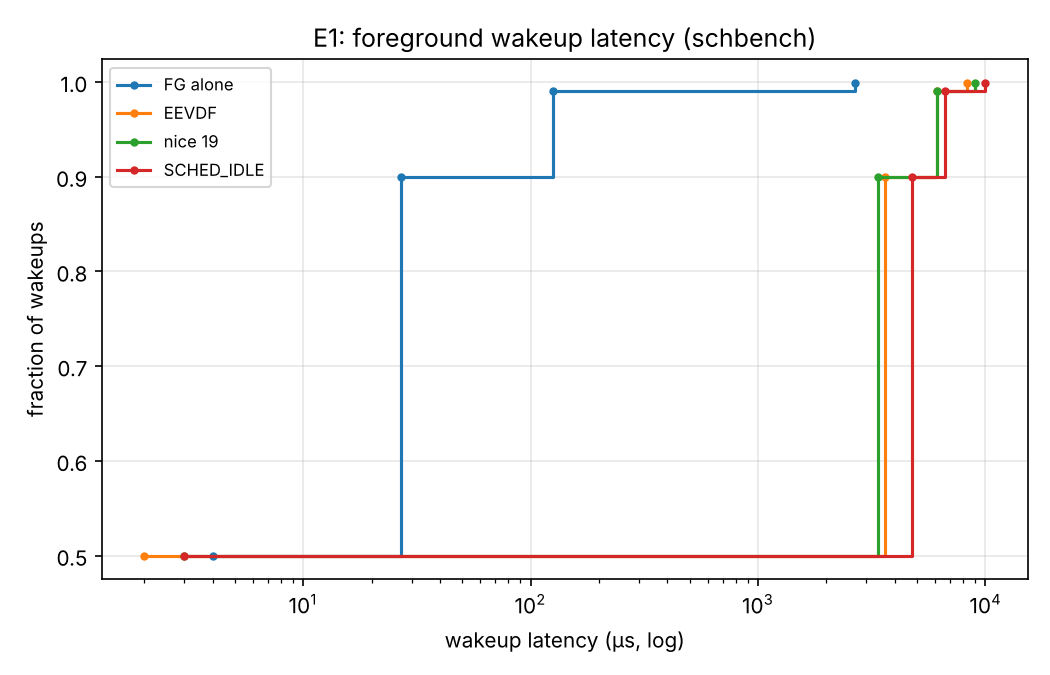
\includegraphics[width=0.72\linewidth]{figures/fig1_e1_latency_cdf.png}
\caption{E1: schbench wakeup-latency distribution per baseline, from schbench's percentile points (median over repetitions). Background load moves the tail from about 0.1\,ms to about 6\,ms, and lowering its priority does not move it back.}
\label{fig:e1}
\end{figure}}{}

\IfFileExists{figures/fig2_e2_jitter_box.png}{%
\begin{figure}[t]
\centering
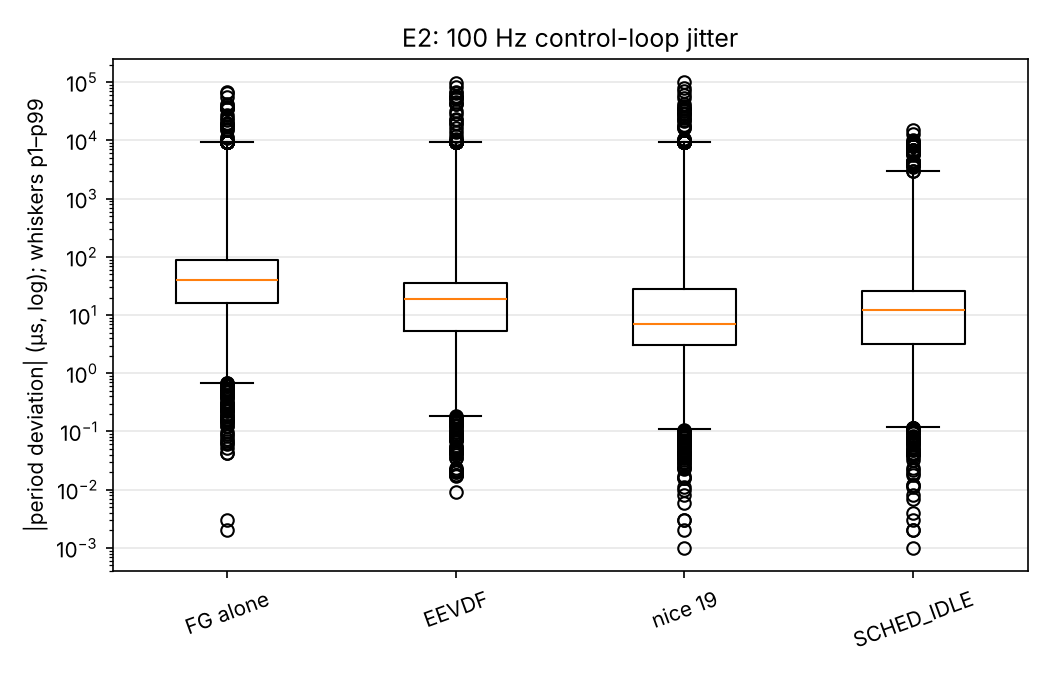
\includegraphics[width=0.75\linewidth]{figures/fig2_e2_jitter_box.png}
\caption{E2: distribution of $|$period deviation$|$ of a 100\,Hz loop under each baseline (all repetitions pooled). The foreground-alone reference is itself noisy on this virtual machine, so this experiment is inconclusive here.}
\label{fig:e2}
\end{figure}}{}

\paragraph{Observations.}
With CPU-bound background load at the same priority (B1), the p99 wakeup latency of schbench rose to 48.6$\times$ the foreground-alone value (B0). Background at nice~19 (B2) gave 48.8$\times$ and \code{SCHED\_IDLE} (B3) 52.5$\times$ (\cref{tab:e1}).
E2 is inconclusive on this machine. The 100\,Hz loop running \emph{alone} (B0) already showed a p99 period deviation of 9.4\,ms and a maximum of 66\,ms (\cref{tab:e2}), i.e.\ the virtual machine's timer and vCPU scheduling dominate the jitter, so differences between B1--B3 cannot be attributed to the background priority mechanism. E2 must be repeated on bare metal.
Background progress was similar across B1--B3 (79--90 CPU-seconds per minute in E1 on 4 vCPUs). The question scx\_hush targets is whether strict precedence can bring foreground latency back to B0 at a similar background cost.
These measurements quantify the interference that motivates scx\_hush on this machine; they are not an evaluation of scx\_hush, and the VM's noise (\cref{sec:discussion}) means only large effects should be read from them.


\subsection{scx\_hush results}
E1--E9 for B5 and B6 are \pending. They need a kernel with
\code{CONFIG\_SCHED\_CLASS\_EXT=y}. The PRD's targets, against which those
results will be judged, are:
\begin{itemize}
\item foreground p99 latency within $1.2\times$ of foreground alone, and
  throughput at least 90\% of foreground alone;
\item background using at least 80\% of the idle CPU share;
\item no background wait longer than the guard interval;
\item a lock holder blocking foreground for at most one boost slice after
  detection;
\item under 2\% overhead with no background work;
\item zero watchdog aborts in a 24-hour soak.
\end{itemize}

\section{Gaps Fulfilled}
\label{sec:gaps}

\Cref{tab:gapmap} maps each research gap from \cref{sec:related} to the
mechanisms that address it, and states how the claim is or will be supported.

\begin{table}[h]
\centering\small
\caption{How scx\_hush addresses the identified gaps.}
\label{tab:gapmap}
\begin{tabularx}{\linewidth}{@{}lXl@{}}
\toprule
Gap & Mechanism in scx\_hush & Evidence \\
\midrule
G1 & Strict DSQ order, preemption kick plus tick backstop; per-CPU rate-limited guard with a watchdog-safe hard guard & design; E1, E4, E6 \pending \\
G2 & Policy-driven classes (cgroup, comm, uid), fork inheritance, exec/rename re-classification; no application changes & implemented, tested \\
G3 & PI-futex and glibc-mutex owner detection in the kernel; hints optional; same-process fallback & implemented; E5 \pending \\
G4 & All logic in verified BPF; \code{sched\_ext} fallback; guard $\le W/4$ enforced; API isolation (NFR-9) & implemented; E8 \pending \\
G5 & One harness for B0--B6 and E1--E9 with raw CSV, metadata and bootstrap CIs & implemented; baselines measured \\
\bottomrule
\end{tabularx}
\end{table}

\section{Discussion and Limitations}
\label{sec:discussion}

\paragraph{Threats to validity.}
The baselines were measured on a shared virtual machine, where hypervisor
scheduling adds noise that bare metal would not have. Short runs (20\,s) and
three repetitions give wide confidence intervals. On this VM, the foreground-alone 100\,Hz loop (E2, B0) already
missed deadlines by up to tens of milliseconds, so jitter experiments can only
be judged on bare metal. The final campaign should
use bare metal, pinned frequency, five repetitions of 120\,s, and a real
kernel build as background load, as the methodology specifies.

\paragraph{Known limitations.}
\begin{itemize}
\item Locks shared across processes through shared memory are detected only by
  tier~1.
\item Spinlocks and lock-free retry loops are invisible to every tier; only
  the guard protects against them.
\item Tier~3 depends on glibc's mutex layout and is disabled when the
  self-test fails.
\item Owner lookup uses the initial PID namespace, which limits tiers~2--3
  inside containers.
\item A single global \code{BG\_DSQ} may contend beyond 16 CPUs; E7 will tell
  whether it needs sharding.
\end{itemize}

\section{Conclusion and Future Work}
\label{sec:conclusion}

scx\_hush gives general-purpose Linux machines strict foreground isolation
with bounded background starvation and in-kernel priority-inversion handling,
without application changes. It is deployed safely through \code{sched\_ext}.
We contributed a gap analysis, a design that closes a watchdog-safety hole
left by per-CPU rate limiting alone, a complete implementation, and a
reproducible evaluation methodology. Baseline measurements (E1) show that
the existing Linux priority mechanisms leave a roughly $49\times$ tail-latency
penalty under background load, which is the interference scx\_hush is
designed to remove.

The immediate next step is to run E1--E9 on a \code{sched\_ext}-enabled kernel
on bare metal and on embedded boards. That will test verifier acceptance and
the PRD's quantitative targets, and answer the open design questions: whether
NORMAL should also be preemptible by FOREGROUND, whether \code{BG\_DSQ} needs
sharding, and whether kick latency stays below 100\,$\mu$s.

\bibliographystyle{plain}
\bibliography{refs}

\end{document}
